
{

\Hide
\chapter{Resultados y discusión}
}

\begin{titular} 
	\uppercase{
	capítulo 4 \\
	Resultados y discusión \\
	}
\end{titular}

\section{Mapeo sistemático}

En respuesta a RQ1 y  RQ 2, en el mapeo sistemático identificamos 101 estudios publicados entre 
2003 y 2013 que planteaban algún modelo, propuesta o implementación de un sistema de votación 
electrónica.  De los cuales 60 mencionaban explícitamente la consideración de algún 
requerimiento no funcional enmarcado dentro de las subcaracterísticas presentadas en el estándar
de calidad de software ISO/IEC 25010. 

\begin{table}[h!]
\centering
\caption{Nº de estudios según subcaracterísticas de NFR}
\label{tab:estudios-subcaracteristicas}
\begin{tabularx}{0.8\textwidth}{X c r} 
\toprule[1.5pt]
	\bf	Subcaracterística	& 	\bf Frecuencia	& \bf Porcentaje \\ 
	Confidentiality			&	18			& 30.00\% \\
	Resource utilisation		&	14			& 23.34\% \\
	Fault tolerance			&	5			& 8.30\% \\
	Integrity 				&	4			& 6.67\% \\
	Non-repudiation		&	3			& 5.00\% \\
	Ease of Use			&	2			& 3.34\% \\
	Authenticity			&	2			& 3.34\% \\
	Security Compliance	&	2			& 3.34\% \\
\bottomrule[0.5pt]
\end {tabularx}
\end{table}
\bigskip

En respuesta a RQ 2.1, de los 19 los requerimientos no funcionales revisados en los estudios
seleccionados, fueron encontrados sólo 8: Non-repudiation, Fault tolerance, Resource behavior, Ease of Use, 
Confidentiality, Integrity, Authenticity y Security Compliance. Los resultados son consistentes 
con la literatura analizada en capítulos anteriores ya que como se refleja 
en la Figura~\ref{fig:chart-caracteristicas}, existe una presencia predominante de aspectos
asociados a protocolos criptográficos: seguridad y recursos computacionales necesarios para 
ejecutarlos.

\begin{figure}[h!]
	\centering
	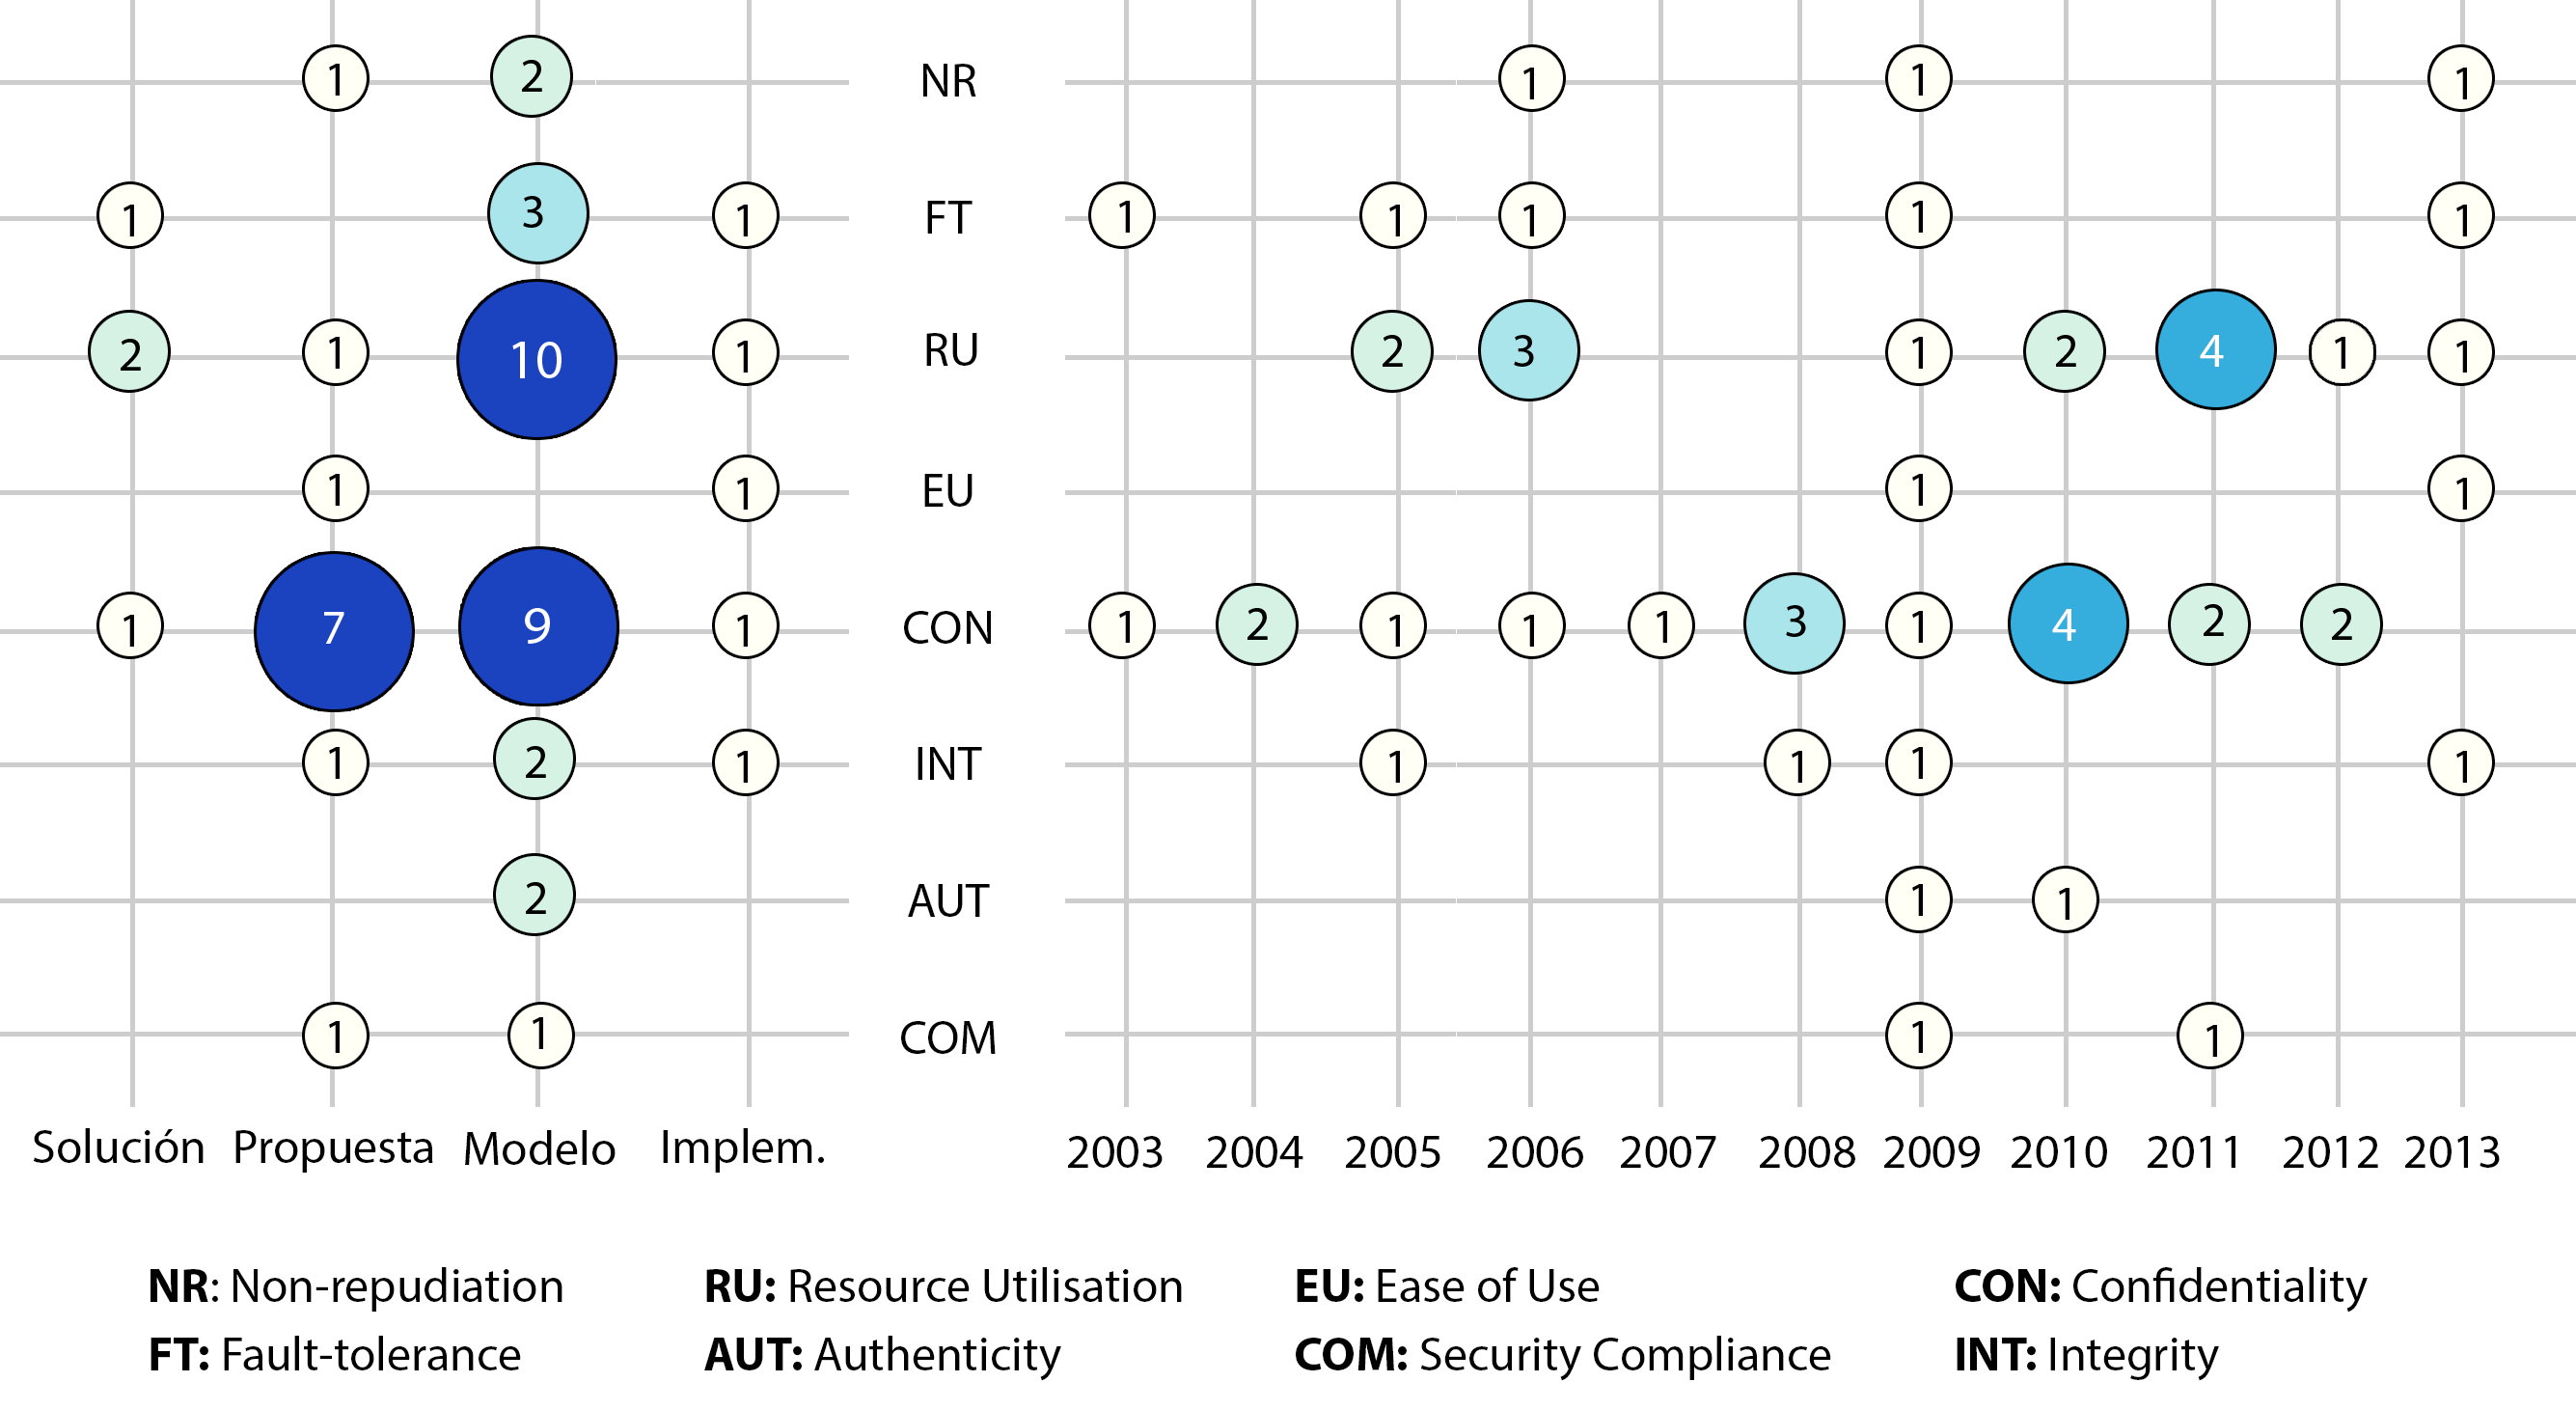
\includegraphics[width=\textwidth]{figura-mapafinal1}
	\caption{Mapa de subcaracterísticas de ISO/IEC 25010 en modelos e 
	implementaciones de sistemas de votación electrónica}
	\label{fig:mapa-final1}
\end{figure}
\bigskip


El producto final del mapeo sistemático fue dividido en 2 figuras por restricciones de espacio. La
figura~\ref{fig:mapa-final1} muestra todos los estudios que fueron clasificados en sólo una categoría
mientras que la figura~\ref{fig:mapa-final2} muestra los que fueron clasificados en múltiples categorías.
Revisando las dos figuras, se desprenden varias conclusiones: los trabajos mayoritariamente 
plantean modelos y sólo una pequeña parte presenta implementaciones de sistemas de votación 
electrónica.  

El detalle de todos los estudios incluidos en la clasificación final están
incluidos en el apéndice. El anexo A incluye la puntuación de cada publicación
mientras que el anexo B incluye los datos de todas las publicaciones seleccionadas
en el mapeo sistemático.

\begin{figure}[h!]
	\centering
	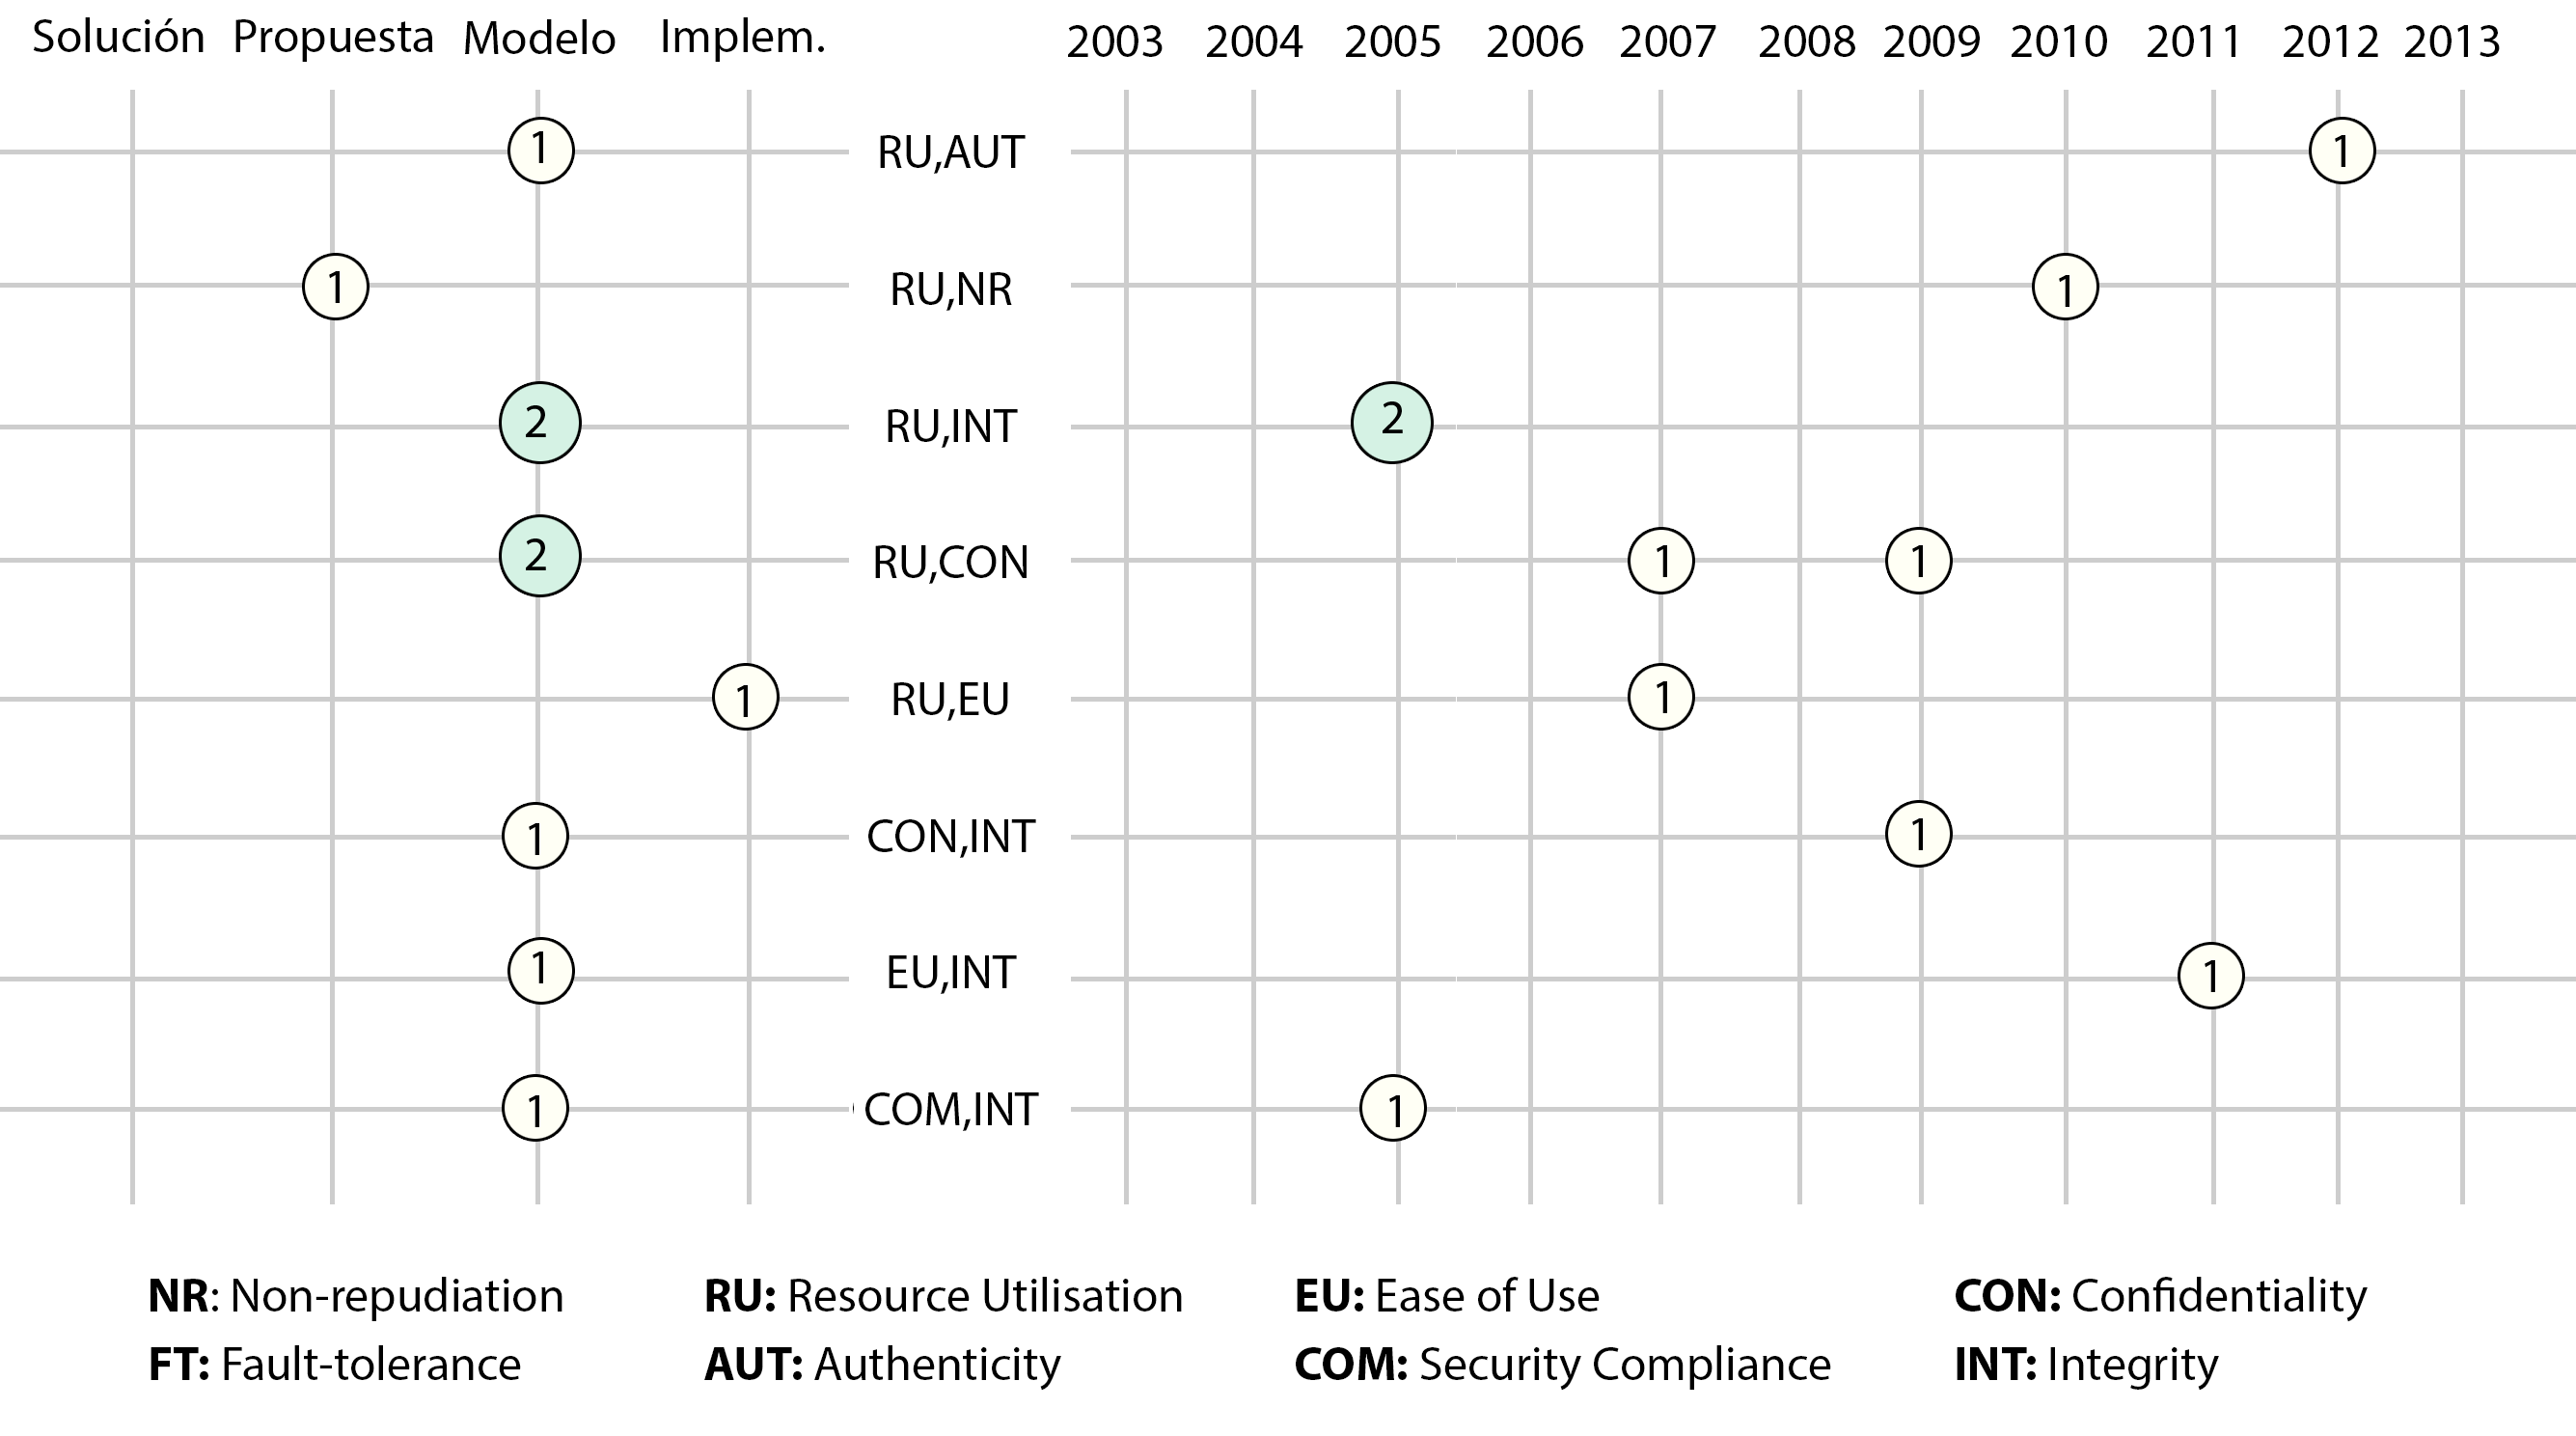
\includegraphics[width=\textwidth]{figura-mapafinal2}
	\caption{Mapa de múltiples subcaracterísticas de ISO/IEC 25010 en modelos e 
	implementaciones de sistemas de votación electrónica}
	\label{fig:mapa-final2}
\end{figure}
\bigskip

En la figura~\ref{fig:mapa-final2} se desprende la poca cantidad de trabajos que
explícitamente aborda más de algún requerimiento no funcional en la votación electrónica. 
De los trabajos que se encontraron, se revela que la subcaracterística que más
se conjuga con otras es Resource Utilisation, seguido por Integrity, lo cual es consistente
con lo dicho anteriormente que son los aspectos inherentes de los protocolos criptográficos
los que se ven reflejados en los requerimientos no funcionales.

\newpage
\section{Evaluación y amenazas a la validez}

Después de haber conducido la búsqueda, se evaluó qué tan legítimo son 
nuestros resultados y consideramos que existen 2 amenazas a la validez: 
\textit{la elección de las subcaracterísticas del ISO/IEC 25010:2011} y 
\textit{la ausencia de trabajos indexados en Springer Link} 


\begin{itemize}
	\item \textbf{Elección de subcaracterísticas:} No se eligió revisar las 27 
	características del ISO/IEC 25010:2011 en todas las publicaciones principalmente
	por restricciones de tiempo. La elección de las subcaracterísticas está 
	respaldada por distintos trabajos, aún cuando no existe en la literatura alguno
	que defina formalmente las subcaracterísticas que más importan en los 
	modelos de votación electrónica.
	
	\item \textbf{Ausencia de trabajos indexados en Springer Link:} Existe una
	importante cantidad de trabajos relativos a la votación electrónica que se encuentran
	únicamente indexados en esta biblioteca digital. Una búsqueda informal arrojó
	varios trabajos que podrían haber sido incluidos en la selección final, en especial
	varios libros de la serie \textit{Lecture Notes on Computer Science}(LNCS). La justificación
	de no incluir SpringerLink se debe a la dificultad de ejecutar búsquedas lógicas
	y de acceder a los trabajos que están alojados. 
	
\end{itemize} 

\section{Discusión}

Dada la cantidad de modelos y la cantidad de sistemas propuestos en la
literatura, está claro que la votación electrónica es una área con bastante
actividad científica enfocada en la propuesta de modelos que puedan resolver
los problemas que están presentes en la satisfacción de los requisitos
dados por las votaciones tradicionales. 

\begin{figure}[h!]
	\centering
	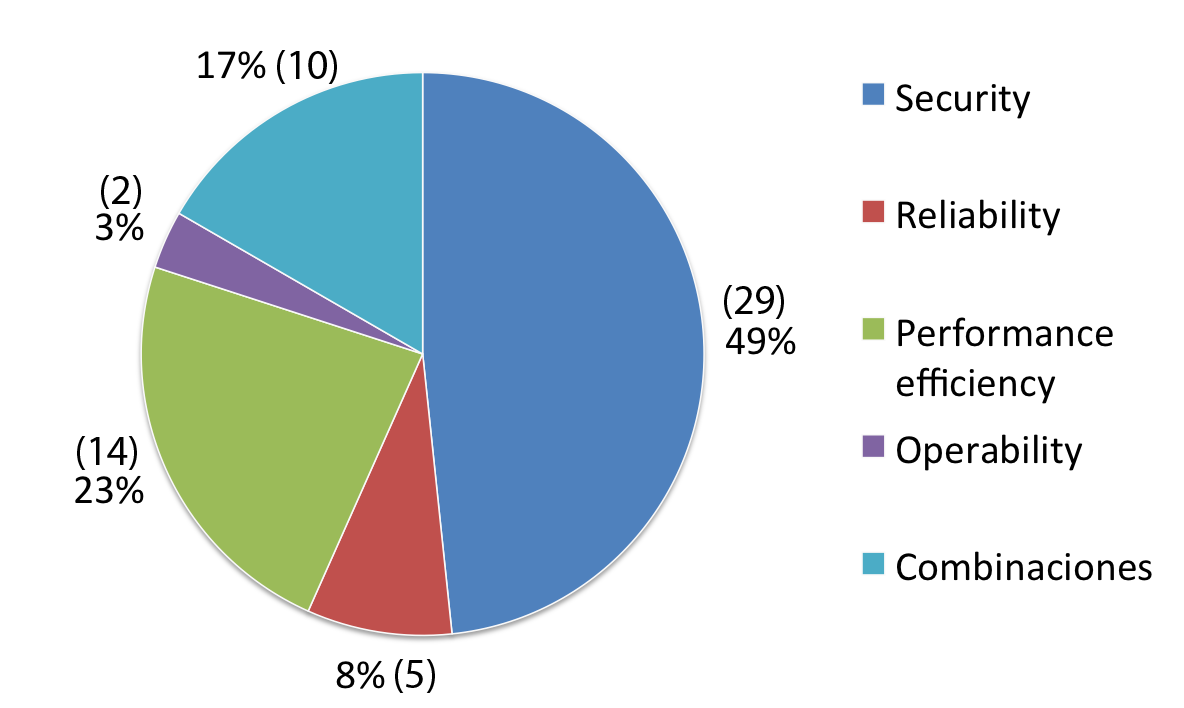
\includegraphics[width=0.7\textwidth]{figura-chart-caracteristicas}
	\caption{Distribución de las publicaciones según característica de calidad ISO/IEC 25010}
	\label{fig:chart-caracteristicas}
\end{figure}
\bigskip

Que la mayor cantidad de estudios se enfoque en los aspectos de seguridad
de los sistemas de votación electrónica demuestra lo crítico que es para el
éxito en la adopción de estos sistemas que sean dignos de confianza y puedan
asegurar el cumplimiento de los requerimientos legales de las votaciones 
alrededor del mundo. Pese a que la seguridad es la mayor prioridad, preocupa
que, como ha señalado \cite{Al-Shammari2012}, varios sistemas de votación 
electrónica que actualmente han sido utilizados sufren de serias fallas de diseño
e implementación y son vulnerables a ataques maliciosos. 


Considerando que una de las características del sufragio universal es que todas las 
personas mayores de cierta edad pueden ejercer su derecho a voto, resulta sorprendente
que de los trabajos se revela que la accesibilidad es un tema que no está presente
en las propuestas de sistemas de votación electrónica. Actualmente ningún sistema de 
votación sirve completamente a todos los votantes, incluyendo quienes tienen 
discapacidades, y reportes de algunas elecciones 
que incluyen sistemas electrónicos equipados con interfaces accesibles no son
implementados o son implementados de manera incorrecta en los lugares de votación
es problemático. \cite{Goodman2012}

De la figura~\ref{fig:chart-caracteristicas} se revela que los esfuerzos están 
puestos en formular e implementar algoritmos y modelos de seguridad comprobada. Si bien
se entiende que para el e-voting la seguridad es crítica, ¿Por qué existen tan pocos trabajos en 
otros aspectos de calidad? Una posible explicación de la actual situación de los sistemas de votación electrónica
es que simplemente no es posible hacerlo de forma segura: "Todas las elecciones
nacionales (en E.E.U.U.) desde el 2000 nos ha mostrado lo mismo: los sistemas de votación 
fallan frecuentemente. Y cuando fallan, los votos son perdidos. (...) Esto no es aceptable. El 
derecho a voto es el derecho constitucional más fundamental'' \cite{Goodman2012}. Si aún
no se resuelven los temas de seguridad difícilmente se puede enfocar en otros aspectos
de calidad de software.

\begin{figure}[h!]
	\centering
	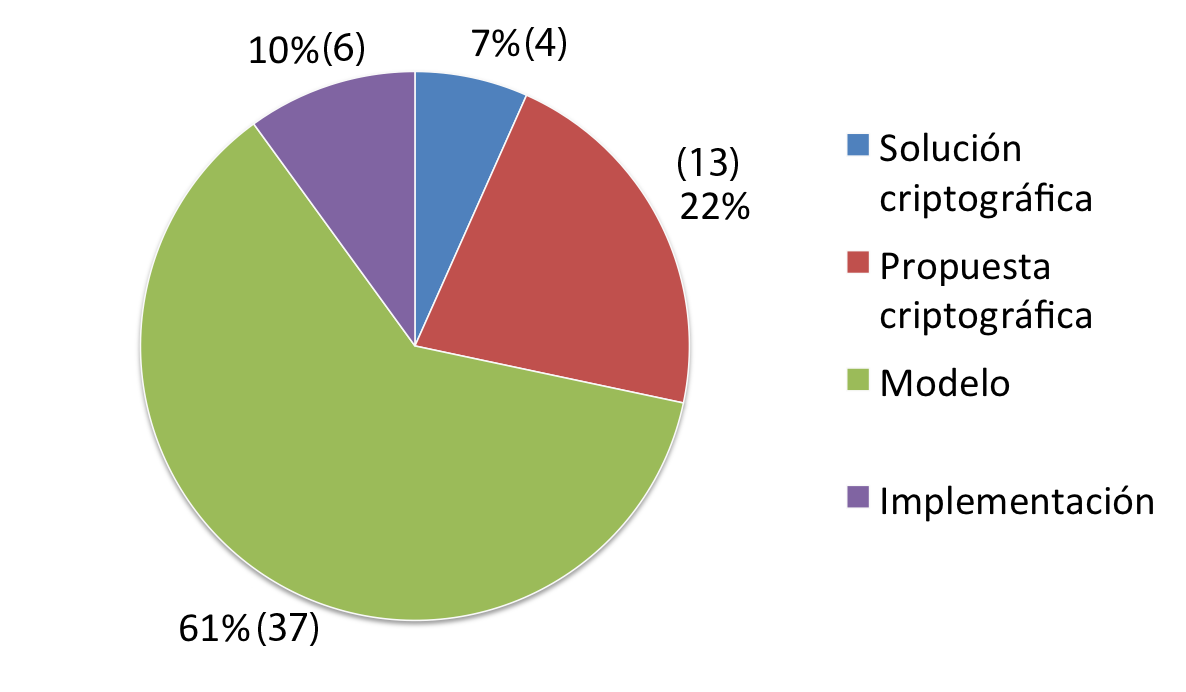
\includegraphics[width=0.7\textwidth]{figura-chart-clasificaciones}
	\caption{Distribución de las publicaciones según tipo de propuesta}
	\label{fig:chart-clasificaciones}
\end{figure}
\bigskip

Los estudios revisados indican que en general la aplicación de modelos de calidad a la propuesta
e implementación de sistemas de e-voting es una área inmadura, revisando los últimos 10 años
encontramos que la mayoría de las publicaciones son modelos teóricos. Si bien los desafíos de
la votación electrónica están bien establecidos, cuando buscamos soluciones en la literatura
encontramos principalmente propuestas, puesto que sólo un 10\% de los trabajos revisados 
reporta uso, implementación y/o evaluación de las propuestas, tal como lo ejemplifica 
la figura~\ref{fig:chart-clasificaciones}. Una posible explicación de este fenómeno es
que los sistemas de e-voting suelen ser de código cerrado, y sólo algunas personas tienen acceso
a información detallada acerca de cómo funcionan.  \cite{Benoist2007} indica que
faltan esfuerzos en construir programas de código abierto, en simplificar la implementación 
de sistemas y mejorar la transparencia de hardware para poder conseguir que la votación 
electrónica sea una aplicación exitosa de tecnología.

La eficiencia es un aspecto que varios estudios toman en cuenta, pero con 
distintos puntos de vista puesto que algunos lo utilizan para hacer su protocolo/esquema
práctico, en el sentido de que \textit{es posible} usarlo en votaciones reales
mientras que otros se enfocan explícitamente en votaciones a gran escala. Entonces, aparece 
el problema de proveer una solución que satisfaga la
definición de seguridad más fuerte o encontrar protocolos eficientes que puedan
ser implementados a gran escala. Algunos estudios abordan esta temática
pero en general no está planteado, por una parte por la falta de implementaciones
libres o de código abierto que se utilicen e incorporen mejoras propuestas
por la literatura.


\newpage
\section{Recomendaciones}

\begin{enumerate}

	\item Dados los resultados del mapeo sistemático, proponemos una jerarquización dentro de las 8 
		características del modelo de calidad ISO/IEC 25010, esto para poder enfocar los esfuerzos
		de futuras propuestas. La figura~\ref{fig:concentrico} muestra las 8 características, siendo
		la prioridad máxima el \textit{security}, seguido en segundo lugar \textit{Reliability}, \textit{Operability}
		 y \textit{Performance Efficiency}, para dejar en tercer lugar \textit{Maintainability},\textit{Portability},
		\textit{Functional Suitability} y \textit{Compatibility}.

	\begin{figure}[h!]
		\centering
		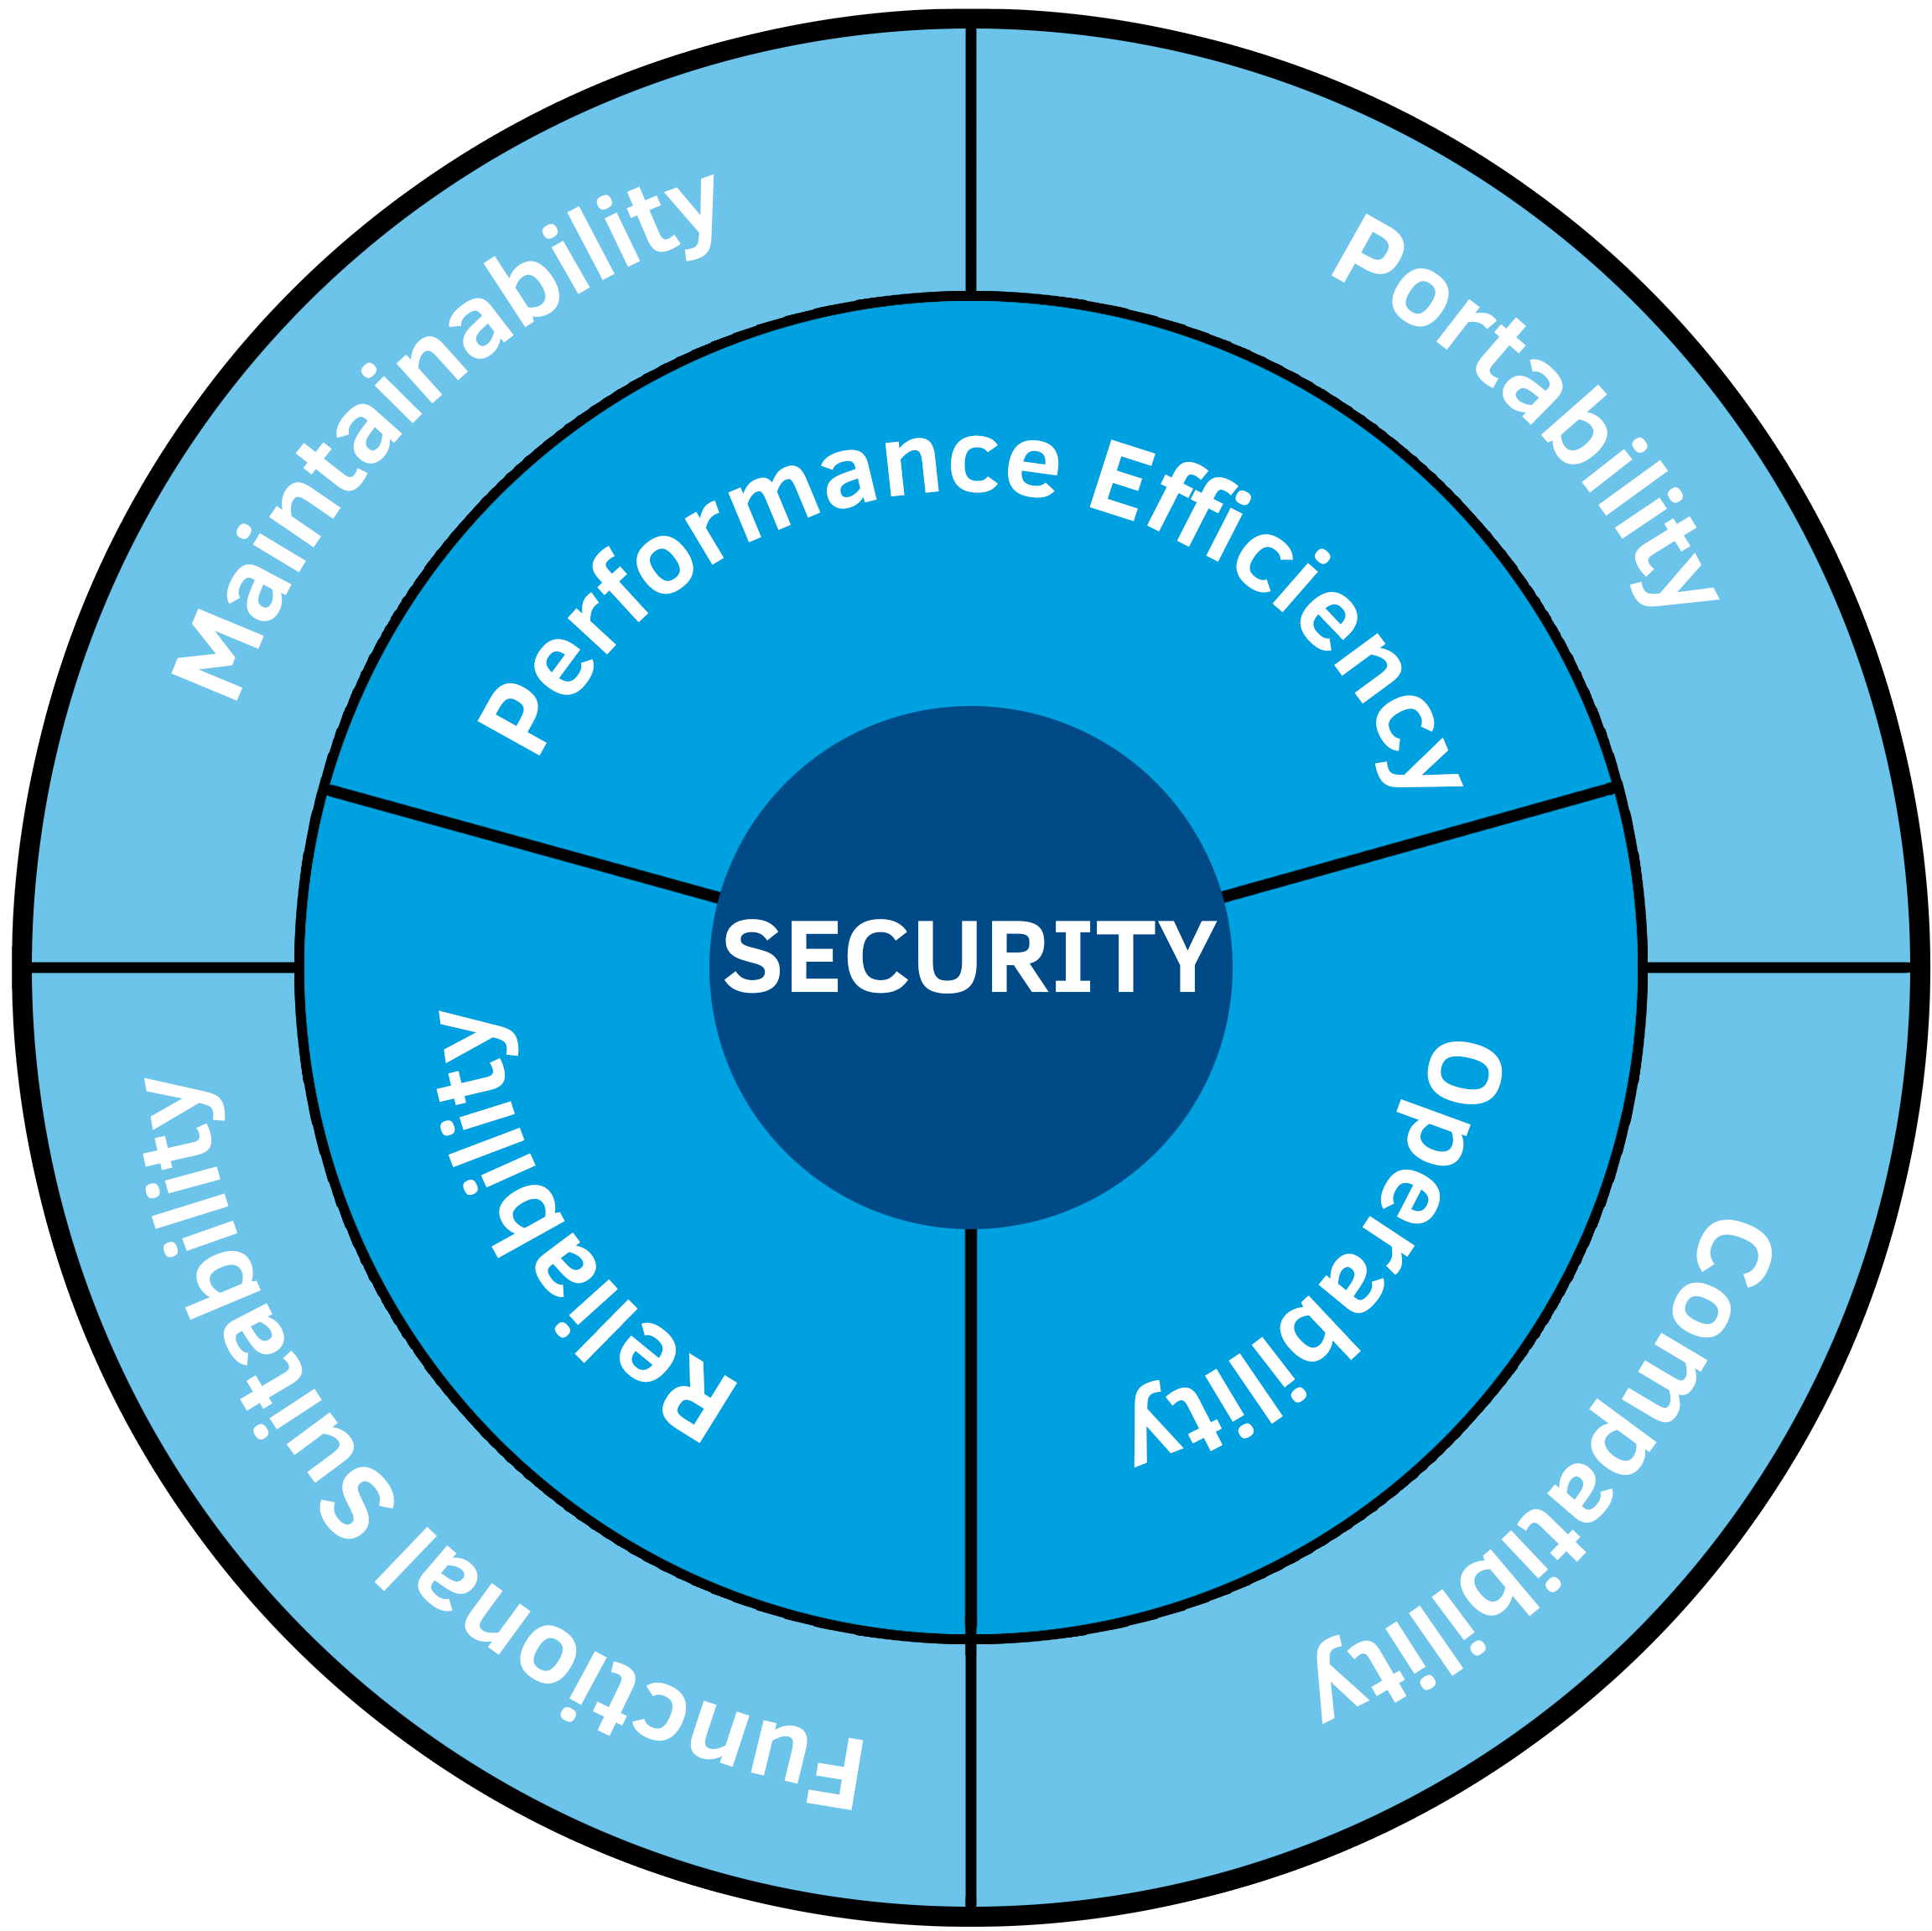
\includegraphics[width=0.5\textwidth]{figura-concentrico}
		\caption{Jerarquización de las características ISO/IEC 25010 en modelos de votación electrónica}
		\label{fig:concentrico}
	\end{figure}
	\bigskip
		
		El objetivo que tiene esta jerarquización es la de orientar los futuros modelos e implementaciones
		de sistemas de votación electrónica a construir software que genere \textit{confianza}. La seguridad
		por sí sola no lo asegura, puesto que como plantea \cite{Spycher2012} algunas suposiciones de seguridad
		hacen impracticables los protocolos en elecciones de gran tamaño.
		
		Los sistemas de votación electrónica deben generar confianza, tanto en los gobiernos que lo implementan
		como en los ciudadanos que lo usan. Para generar confianza se recomienda 
		tener \textit{security} como eje principal, es decir, partir construyendo el modelo 
		buscando garantizar la integridad del sistema, luego en segundo lugar aparecen 3 características:		
		\textit{Performance Efficiency} y \textit{Reliability}  están para que el software sea adecuado cuando se utiliza en elecciones a gran escala, 
		\textit{Operability} está para poder garantizar que todos los usuarios puedan hacer uso del software 
		con la menor necesidad de ayuda externa.
	

	\item Construir y mantener sistemas de votación electrónica usando software de código abierto. El utilizar código
		abierto tiene 2 finalidades: transparencia y seguridad. Actualmente los sistemas de votación electrónica
		son de código cerrado, es decir, usualmente sólo personas que pertenecen a la organización encargadas 
		de mantener el software	tienen acceso al código fuente y a los servidores utilizados. Esto implica que los 
		ciudadanos pierden cierto control sobre el proceso eleccionario, puesto que pueden insinuar que el
		software puede manipular el resultado. Si el software estuviese abierto al escrutinio público, nadie podría
		sugerir que tiene trampas u omisiones, ademas de que cualquier entidad interesada
		en examinar el software y encontrar bugs, los cuales pueden ser corregidos e 
		incorporados rápidamente.
		
		Actualmente varias naciones licitan máquinas y software a sólo una empresa, por lo que 
		es posible que queden "amarradas" (vendor lock-in) a la tecnología que la empresa haya
		decidido utilizar. Usando código abierto es posible disminuir la dependencia a una sola entidad
		puesto que es posible integrar tecnologías de distintos vendedores. \cite{Langer2010}

		
	\item Abordar el problema de la votación electrónica de forma holística, buscando detectar y formalizar problemas que aparecen al incluir en los modelos e implementaciones
		no sólo aspectos de seguridad, sino otras características que están en los modelos de
		calidad de software como son Reliability, Usability, Maintainability y Portability. Incluso en
		casos de éxito como en países como Estonia, serios problemas de seguridad relativos
		a la administración revelan si el nivel actual de los sistemas de votación electrónica
		son útiles para la adopción futura en otras naciones.\cite{Schryen2009} 
		
		Si bien el construir sistemas electrónicos debería ser un tema esencialmente tecnológico,
		al ser la votación algo fundamentalmente político, al adoptar estos sistemas se debe 
		considerar el factor humano.	Desde una perspectiva ortogonal existen avances en las distintas capas del proceso 
		eleccionario, pero al ampliar la mirada a todos los componentes aparecen problemas
		como la imposibilidad de garantizar que todos los ciudadanos, incluyendo discapacitados
		y ancianos, sean capaces de votar en sistemas de votación puramente electrónicos. Es por esto
		que se recomienda al plantear modelos y/o implementaciones de votación electrónica 
		ampliar su alcance para que cubra todas las capas del proceso eleccionario.	
		
		En la ingeniería de software encontramos la modelación basado en objetivos como una herramienta
		en dirección a una visión holística del problema de la votación electrónica, donde se pueden
		abordar tanto factores humanos como tecnológicos. En la figura~\ref{fig:diagrama-sd} se modela
		un sistema de votación electrónica utilizando la notación i* (i star).
		
\begin{figure}[h!]
	\centering
	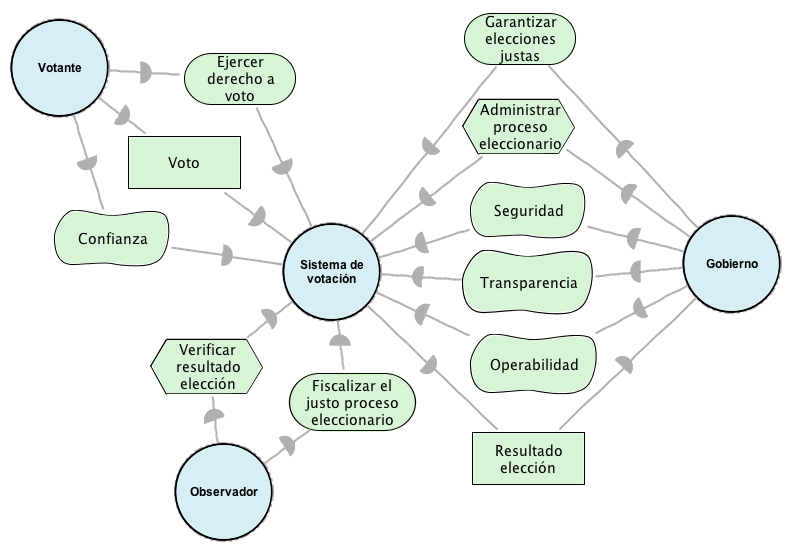
\includegraphics[width=\textwidth]{figura-diagrama-sd}
	\caption{Diagrama i* SD system-to-be de un sistema de voto electrónico}
	\label{fig:diagrama-sd}
\end{figure}
\bigskip

		En el diagrama se identifican 4 actores: El gobierno, el votante, el observador y el sistema de votación. El
		gobierno se refiere a cualquier entidad o persona involucrada con la administración del proceso eleccionario. El 
		votante se refiere a los ciudadanos. El observador se refiere a cualquier entidad independiente del gobierno y el
		sistema de votación se refiere al conjunto de software, hardware y recursos humanos que sirven como medio
		para poder realizar el proceso eleccionario. 
		
		Los \textit{hard goals} están relacionados directamente con los requisitos de la votación electrónica anteriormente
		mencionamos mientras que los \textit{soft goals} están relacionados con los atributos de calidad recomendados.
	
\end{enumerate}
